\section*{\centering ABSTRACT}
Bas-relief is an art form part way between 3D sculpture and 2D painting. We present a new approach for generating a bas-relief from a single Chinese brush painting.We do not aim to recover exact depth of a painting, which is a tricky computer vision problem, requiring assumptions that are rarely satisfied.Instead, our approach exploits the concept of brush strokes, making each brush stroke possible to generate a correspond bas-relief proxies(depth map of brush strokes),and combine the depth map of brush strokes together to construct the bas-relief model. To segment brush strokes in 2D paintings, we reformulate layer decomposition and stroke segmentation by imposing boundary constraints, which can make strokes smooth and complete. The resulting brush strokes are sufficient to evoke the impression of the consistent 3D shapes on bas-relief, so that they may be further edited in 3D space. This fulfills the request of recomposition in bas-relief design. Currently, our research focus on Chinese brush paintings with relatively sparse strokes. We demonstrate our approach on a variety of Chinese brush paintings, and even some other suitable styles include rosemaling paintings and certain watercolor paintings, our approach is able to produce convincing bas-reliefs.



\begin{figure}[H]
\centering
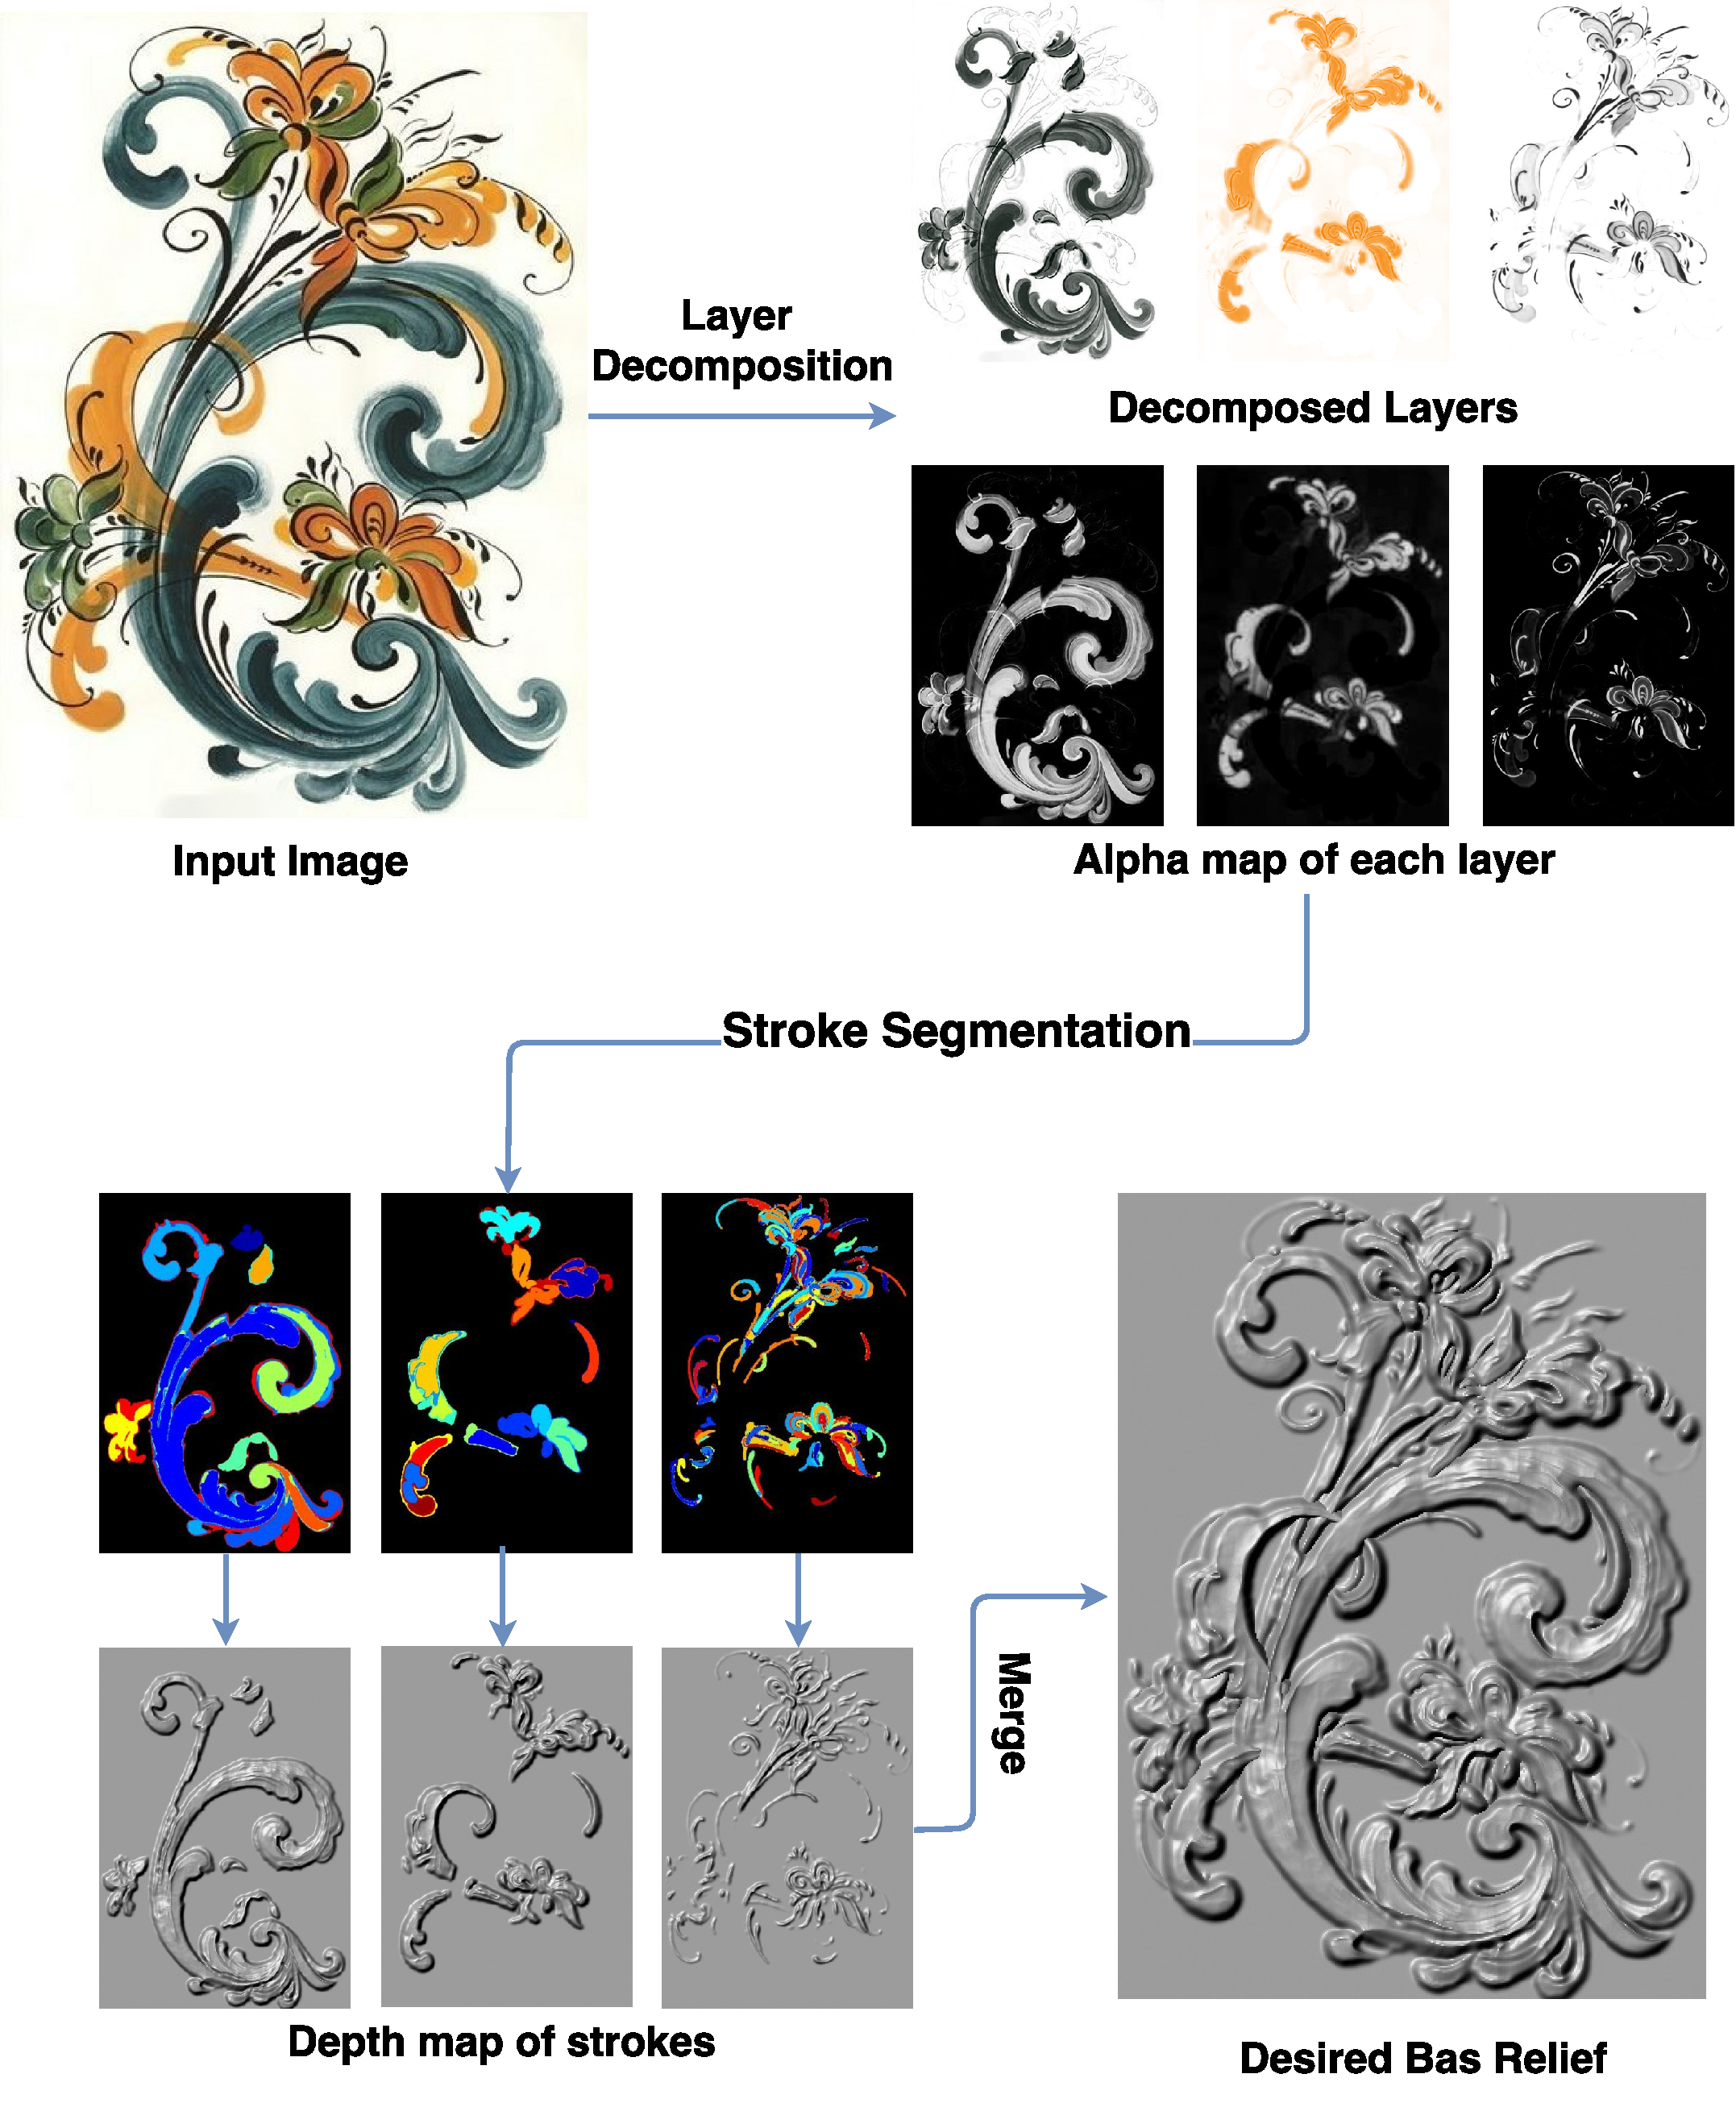
\includegraphics[scale=0.4]{overview.pdf}
\caption{Pipeline Overview}
\label{pip}
\end{figure} 
 
\newpage


 

